\setchapterpreamble[u]{\margintoc}
\chapter{Trattamenti termici}
\labch{cap9}

Si è visto nel capito precedente che i passaggi di fase dipendono sia dalla temperatura che dal tempo della sua variazione. È quindi evidente che variando il tempo di raffreddamento o di riscaldamento si otterranno risultati molto diversi. I processi termici sono caratterizzati da un riscaldamento e da un successivo raffreddamento, lento o veloce.

\section{Riscaldamento}

Riscaldando si deve arrivare a \textbf{completa austenitizzazione} se la composizione è esattamente eutettoidica (0,8 \%C a 723°C).
Per non deturpare il pezzo durante il riscaldamento ed evitare l’ossidazione\sidenote{Questo problema non si pone se il pezzo in questione è grezzo, ossia deve ancora subire delle lavorazioni. In questo caso lo strato ossidato verrà semplicemente rimosso in seguito.} (a causa della presenza dell’ossigeno che è un inquinante) e la decarbrazione, si utilizzano delle \textbf{atmosfere inerti}\index{atmosfere inerti}.
\begin{enumerate}
    \item \textbf{Gas nobili} quali Argon Ar e elio He, che però hanno un costo non indifferente. Essi si ottengono per distillazione frazionata dell’aria;
    \item \textbf{Azoto N}  che può fungere da gas nobile poiché, in linea di massima, nei trattamenti termici può essere considerato inerte. Solo negli acciai con elevato tenore di cromo Cr non si può utalre tale atmosfera, perché l’azoto reagisce con gli elementi, formando nitruri. L’azoto viene ricavato dall’aria attraverso o la distillazione dell’aria liquida oppure tramite combustione dell’aria (formazione di azoto e di anidride carbonica, l’azoto non reagisce con l’ossigeno). Tali metodi metodi hanno dei costi abbastanza elevati, che variano in base alla purezza dell’azoto.
\end{enumerate}

Tuttavia, si possono avere anche \textbf{atmosfere a basso costo}: noi sappiamo che tale reazione di combustione \mathtext{C_xH_y + O_2 \to CO_2 + H_2O} avviene in eccesso di ossigeno: la \mathtext{CO_2} non è velenosa, a differenza del monossido di carbonio (a meno che non saturi l’atmosfera).\\
Se facciamo avvenire tale reazione in \textbf{rarefazione di ossigeno}, si ha la seguente reazione di combustione:
\mathtext{C_xH_y +O_2 \to CO_2 +H_2O+H_2 +CO}
con i termini a destra che in generale prevengono l'ossidazione. Sono detti \textbf{gas endotermici}\index{gas endotermici}. Si ha infatti la reazione:
\mathtext{CO + H_2O \to CO_2 + H_2} in cui CO e \mathtext{H_2} hanno potere riducente, mentre \mathtext{H_2O\>e\> CO_2} ossidante. \\
Si consideri la reazione: \mathtext{2CO \rightleftharpoons CO_2 +C}, detta \textbf{reazione di Boudoir}. È evidente che il monossido di carbonio possa apportare carbonio al materiale, mentre la \mathtext{CO_2} lo rimuova. Definito il potenziale di carbonio come la concentrazione di carbonio sulla superficie del pezzo in equilibrio con l'atmosfera, risulta chiaro che sia auspicabile (a meno di non voler consciamente variare il contenuto di C della superficie del pezzo, vedi più avanti) avere un potenziale di carbonio uguale alla concentrazione iniziale di C nel pezzo. Si ha che
\begin{equation*}
    \mathtext{p_c}\propto \mathtext{\frac{p^2_{CO}}{p_{CO_2}}}\label{eq:PotC}
\end{equation*}
dove \mathtext{p_{CO}} e \mathtext{p_{CO_2}} sono le pressioni parziali di CO e \mathtext{CO_2} rispettivamente. Siccome questi gas reagiscono secondo la reazione \mathtext{CO + H_2O \rightleftharpoons CO_2 + H_2} si ha
\begin{equation*}
    \mathtext{\frac{p_{CO}}{p_{CO_2}}\propto \frac{p_{H_2}}{p_{H_2O}}}
\end{equation*}
e risulta quindi possibile regolare la pressione parziale di CO e\mathtext{CO_2} tramite quella di idrogeno e vapore acqueo.

Dosando in modo opportuno i generatori endotermici, si riesce ad ottenere un’atmosfera inerte a temperature accettabili, anche se può essere potenzialmente esplosiva, per via della presenza di idrogeno e velenosa, a causa del monossido di carbonio\sidenote{Questo gas è particolamente infame perché, benché sia una sbrega tossico, è inodore, incolore e agisce in maniera graduale. Si lega infatti all'emoglobina, proteina dei globuli rossi incaricata del trasporto di ossigeno, impedendole di svolgere il suo lavoro. Di base, siccome l'uomo come molti altri esseri viventi ha bisogno dell'ossigeno per vivere, questa condizione porta in maniera abbastanza rapida alla morte. Siccome il CO viene prodotto dalle combustioni con una scarsa presenza di ossigeno, gli autori consigliano di non farne in luoghi chiusi (\textit{exempli gratia} accendere il motore dell'auto in garage, fare barbecue in montagna in baita con le finestre chiuse).}. Infatti, quest’ultimo, non avverte della propria presena, perché è incolore e inodore e la sua azione è graduale. Si lega all’emoglobina non lascia tracce.

Dato che si potrebbero avere esplosioni se entrasse ossigeno nel forno, nel forno si ha una \textbf{sovrapressione} rispetto all’atmosfera esterna, facendo sì che l’atmosfera del forno esca in prossimità delle porte di chiusura dei forni, dove prendono fuoco immediatamente.

Si possono avere anche \textbf{trattamenti in vuoto}, che sono anche i più costosi perché la gestione del vuoto è estremamente onerosa. Si devono avere dei forni speciali con pompe per creare il vuoto, con riscaldamenti molto lenti tramite irraggiamento. Questo trattamento sta però diventando sempre più importante perché non inquina dal punto di vista ambientale e quindi evita problemi di tipo legislativo. Con tali trattamenti si eliminano tutti i problemi connessi all’inquinamento, dal punto di vista ambientale e amministrativo.

A volte per velocizzare il processo, il pezzo viene preriscaldato tramite \textbf{azoto} per convezione, e dopo averlo riscaldato, l’azoto viene eliminato e si lavora in vuoto. Il pezzo deve essere pulitissimo, o si corre il rischio di rovinare il forno.\\
In questo tipo di trattamenti si ha il problema della sublimazione di elementi leganti del ferro, se non legati sotto forma di carburi, e quello del raffreddamento, che è preferibile eseguirlo a gas.\\
Il raffreddamento a gas sarà sempre più lento di quello in liquido e possibile solo con acciai alto- legati, che sono molto costosi.\\
Per il \textbf{raffreddamento in liquido}, si utilizza un forno in doppia camera. Si tratta di un tipo di raffreddamento che però si vuole evitare perché il liquido è il maggior inquinante del processo.

Il trattamento in vuoto permette due vantaggi:
\begin{enumerate}
    \item non è inquinante;
    \item permette di ottenere una superficie piatta, cosa ricercata nella produzione di stampi (che devono avere forme perfette).
\end{enumerate}

\subsection{La questione dello Zolfo}

Lo zolfo (S) è generalmente considerato un inquinante nell'acciaio e viene rimosso in fase di produzione (vedi sezione \ref{steel_prod}). In quantità elevate aumenta di molto la fragilità del materiale e ne diminuisce la resistenza. Inoltre abbassa il punto eutettico intorno ai 900°C, rendendo molto più difficili le lavorazioni a caldo per il rischio della formazione di liquido.\\
Viene però aggiunto, in quantità modeste, negli acciai per la lavorazione alle macchine utensili, in combo con del manganese. Insieme formano dei solfuri di manganese, con un punto eutettico oltre i 1200°C, che hanno la proprietà di infragilire il materiale quel tanto che basta per ottenere dei trucioli corti, senza compromettere in maniera significativa le caratteristiche meccaniche. 

\section{Raffreddamento}\label{raffreddamento}

Introduciamo il fattore tempo: se non si dà al sistema il tempo di far avvenire le trasformazioni, cioè se il \textbf{raffreddamento avviene velocemente}, si ha il fenomeno dell’\textbf{isteresi}.\\
Aumentando, quindi, la velocità di raffreddamento, la trasformazione eutettoidica, che avverrebbe a 723°C, si verifica temperature più basse con conseguente variazione dei parametri di diffusione. Se, invece, si \textbf{raffredda lentamente} la temperatura sarà prossima a quella prevista dal diagramma Fe-C, cioè in prossimità della condizione di equilibrio. Ci saranno, quindi, pochi nuclei, poiché la spinta alla trasformazione sarà debole. Tuttavia, tali nuclei crescono molto, in quanto la temperatura è comunque elevata, ottenendo una struttura grossolana caratterizzata da grossi grani, perché la velocità di accrescimento dei nuclei è elevata.

Questa operazione si effettua riscaldando il materiale sopra il punto eutettoidico A3 (di circa 50°C in più) e raffreddandolo lentamente in un forno, sfruttandone l’inerzia termina. Si tratta di un processo costoso chiamato \textbf{ricottura}. La ricottura elimina tutti i trattamenti precedenti e grazie ad essa, si ottiene una struttura grossolana, con poche e grosse lamelle, e fragile (addolcimento del materiale) che può essere lavorata facilmente attraverso lavorazione meccaniche di macchina.

Se si aumenta la velocità di raffreddamento la trasformazione avverrà a temperature via via più basse. Questo comporta una maggior nucleazione e una minor crescita, ottenendo una struttura più fine.

La velocità di raffreddamento può essere aumentata utilizzando il cosiddetto \textbf{raffreddamento in aria calma}, cioè a temperatura ambiente. Questo trattamento è chiamato \textbf{normalizzazione} (50°C al di sopra di \mathtext{A_3} e aria calma).\\
Se non diversamente specificato, i materiali vengono consegnati dopo normalizzazione in quanto è il trattamento più economico, poiché il forno è occupato solo durante il riscaldamento.\\
La struttura finale dipende dalla composizione chimica del materiale, difatti vengono definiti acciai autotempranti quelli che subiscono l’operazione di tempra dopo normalizzazione, e soprattutto dalle dimensioni del pezzo. La struttura finale sarà comunque più fine di quella ottenuta tramite ricottura.

Aumentando ulteriormente la velocità di raffreddamento si ha la \textbf{tempra}, che consiste in un raffreddamento veloce tramite acqua, olio in pressione, soluzioni raffreddanti, liquidi metallici. Con la tempra, si forza notevolmente il sistema e possono accadere due fenomeni anche insieme:
\begin{enumerate}
    \item la soluzione solida di alta temperatura, cioè l’\textbf{austenite}, viene portata a temperatura ambiente, ottenendo acciai austenici, con struttura CFC. E’ il caso degli acciai alto-legati e degli acciai speciali;
    \item si forma una parte di \textbf{austenite residua}, che solitamente è indesiderata perché si trasforma quando il pezzo già è finito, sotto l’azione di lavorazioni meccaniche, con conseguenti dilatazioni volumiche. Essa può essere rimossa con le cosiddette \textbf{operazioni sotto-zero}. Si tratta di lavorazioni che si effettuano in azoto liquido o soluzioni saline sottoraffreddate che hanno lo scopo di eliminare questa parte. Inoltre, si ha il passaggio da una fase CFC ( con costante reticolare a=\mathtext{3,6\cdot10^{-10}}m) a una CCC (a= \mathtext{2,8\cdot10^{-10}m}). Se vi è il tempo giusto, tale trasformazione di schiacciamento e allungamento della cella è facile. Durante tale passagio, il carbonio presente sugli spigoli deve diffondere e formare cementite, ma non gli diamo il tempo: il carbonio, quindi, distorce la struttura facendola diventare tetragonale. Questa configurazione, non prevista dal diagramma Fe-C, è la \textbf{martensite}, struttura estremamente dura a causa dell’alto tenore di carbonio. Essendo una struttura molto dura, è fragile e quindi inutilizzabile. Se si nota una diminuzione di durezza, ciò è dovuto all’austerità residua.
\end{enumerate}

Per ottenere la martensite bisogna impedire le trasformazioni che portano alla formazione di ferrite e cementite, cioè la trasformazione eutettoidica, attraverso un raffreddamento veloce.\\
Lo studio dei trattametni termici può essere effettuato attraverso i \textbf{diagrammi TTT} (Temperature-Time-Transformation) e i \textbf{diagrammi CCT} (Continous-Cooling-Transformation). Questi diagrammi consentono di predire la struttura finale del trattamento termico, e sono quindi fondamentali per progettare tale trattamento.\\
Il digramma TTT predice la struttura che si otterrebbe raffreddando il pezzo, che presenta in partenza una struttura austenitica, alla temperatura voluta in maniera istantanea e mantenendolo in tale stato per un certo periodo di tempo. Il punto individuato da queste due coordinate specifica la struttura cristallina ottenuta a trattamento ultimato. Mantenere l'austenite ad una temperatura alla quale è instabile ne consente infatti la trasformazione, attraverso una \textbf{trasformazione isoterma}.\\
La richiesta che il trattamento venga effettuato a temperatura costante limita l'utilizzo pratico dei diagrammi TTT. Risultano quindi di utilità maggiore quelli CCT.\\
Anche il diagramma CCT presenta le microstrutture in funzione della temperatura e del tempo (in scala logaritmica), ma presentano le curve di inizio e fine trasformazione per raffreddamenti a \textbf{velocità costante} invece che a temperatura costante\sidenote{Esistono diagrammi CCT che rappresentano in ascissa la velocità di raffreddamento del cuore della barra specificando il mezzo in cui avviene il raffreddamento (aria, olio o acqua)}. Questi diagrammi rappresentano meglio situazioni ottenibili in campo industriale rispetto a quelli TTT, e hanno quindi un potere predittivo maggiore. Ciononostante i diagrammi TTT vengono spesso usati al posto dei CCT perché impongono condizioni più stringenti al raffreddamento, garantendo quindi la struttura desiderata a fine processo.\\
Il funzionamento di questi diagrammi è il seguente: tracciata una curva tempo-temperatura che rappresenti il processo di raffreddamento del pezzo, vanno individuate le zone che questa interseca. L'intersezione della linea di inizio trasformazione comporta la formazione di ferrite e cementite sotto forma di perlite o bainite. Siccome queste strutture sono \textbf{stabili} a temperature inferiori a quella eutettoidica, queste non si modificheranno se anche dovessero intersecarsi altre linee. Se persiste dell'austenite residua (ovvero non è stata intersecata la curva di fine trasformazione, che rappresenta una struttura 100\% stabile) questa si trasformerà in martensite. Risulta quindi evidente che, per pter effettuare un processo di tempra che conduca ad una struttura completamente martensitica, la curva di raffreddamento \textbf{non potrà intersecare il ginocchio} della curva di inizio trasformazione.
L'aggiunta di elementi leganti come carbonio, manganese, nichel, molibdeno, cromo o vanadio aumenta la temprabilità dell'acciaio, in quanto sostanzialmente sposta verso destra la pinche curva di inizio trasformazione, consentendo di ottenere la nostra dolce, dolce martensite anche con velocità di raffreddamento minori di quelle richieste per un acciaio al ferro-carbonio puro.\\
Aumentare la dimensione dei grani dell'acciaio ne aumenta la temprabilità: siccome la trasformazione eutettoidica comincia con la nucleazione in punti favorevoli come i bordi di grano, la diminuzione di questi ultimi data da una struttura grossolana rallenta il processo rendendo più facile ottenere martensite pura.\\
\begin{figure}[!hbt]
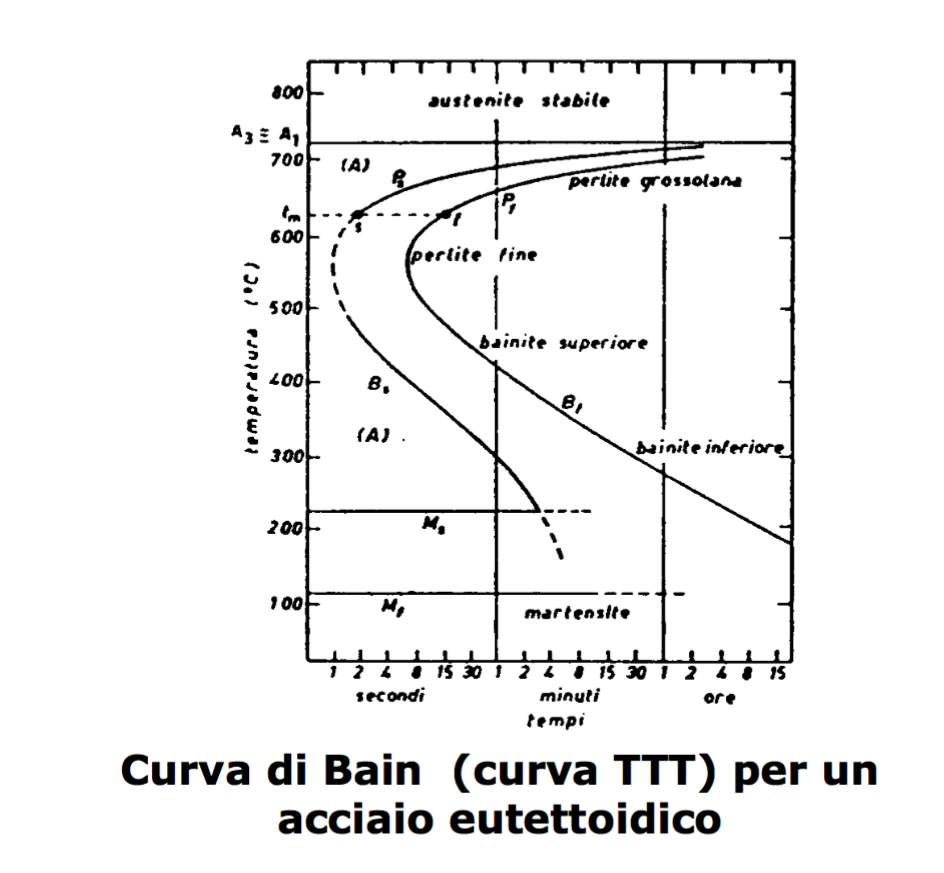
\includegraphics[width=1\textwidth]{images/img32.png}
\caption{Curva di Bain (curva TTT) per un acciaio eutettoidico}
\labfig{img32}
\end{figure}

All'aumentare del tenore di carbonio:
\begin{itemize}
    \item si abbassa la curva \mathtext{M_s};
    \item la trasformazione perlitica viene spostata a destra;
    \item la trasformazione bainitica viene spostata a destra e viene spostata a sinistra la curva di fine trasformazione bainitica, ed aumenta il campo di temperatura in cui è possibile questa trasformazione;
    \item per acciai ipereutettoidici viene anticipata la trasformazione perlitica e non si ha più la trasformazione perlitica.
\end{itemize}

\begin{figure}[!hbt]
    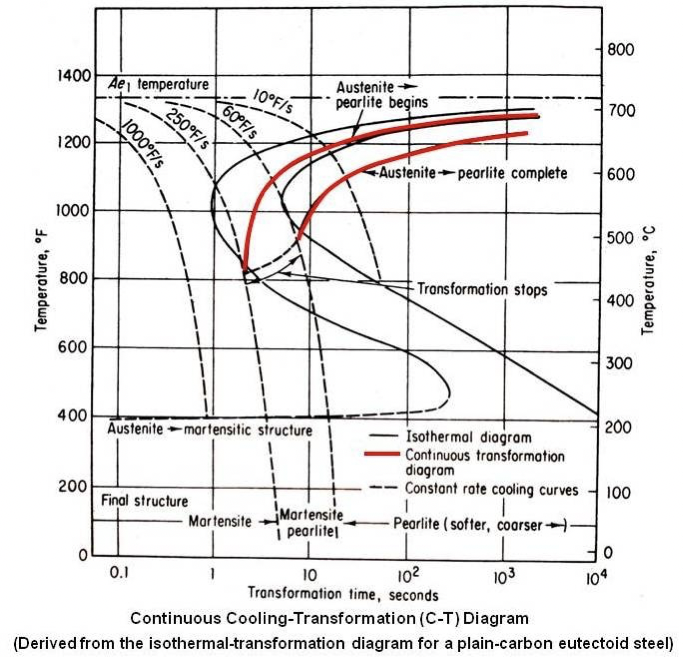
\includegraphics[width=0.6\textwidth]{images/img33.png}
    \caption{Curva CCT per un acciaio eutettoidico}
    \labfig{img33}
\end{figure}

È possibile identificare 3 parti del raffreddamento in un mezzo temprante:
\begin{enumerate}
    \item \textbf{Fase del vapore}: quando la temperatura è molto maggiore della temperatura di evaporazione del liquido temprante si forma una guaina di vapore che circonda il pezzo. Durante questa fase la velocità di raffreddamento è bassa a causa della scarsa conducibilità termica del vapore.
    \item \textbf{Fase di ebollizione}: quando la temperatura si abbassa abbastanza da destabilizzare il film di vapore il liquido evapora direttamente sulla superficie del pezzo. La formazione di bolle comporta una grande turbolenza intorno al pezzo, che viene quindi raffreddato in maniera molto violenta.
    \item \textbf{Fase di convezione}: sotto la temperatura di ebollizione il calore viene asportato principalmente per convezione, dando luogo ad un secondo periodo di bassa velocità di raffreddamento. È possibile aumentare la velocità in questa fase tramite l'agitazione del fluido.
\end{enumerate}

\begin{figure}[!hbt]
    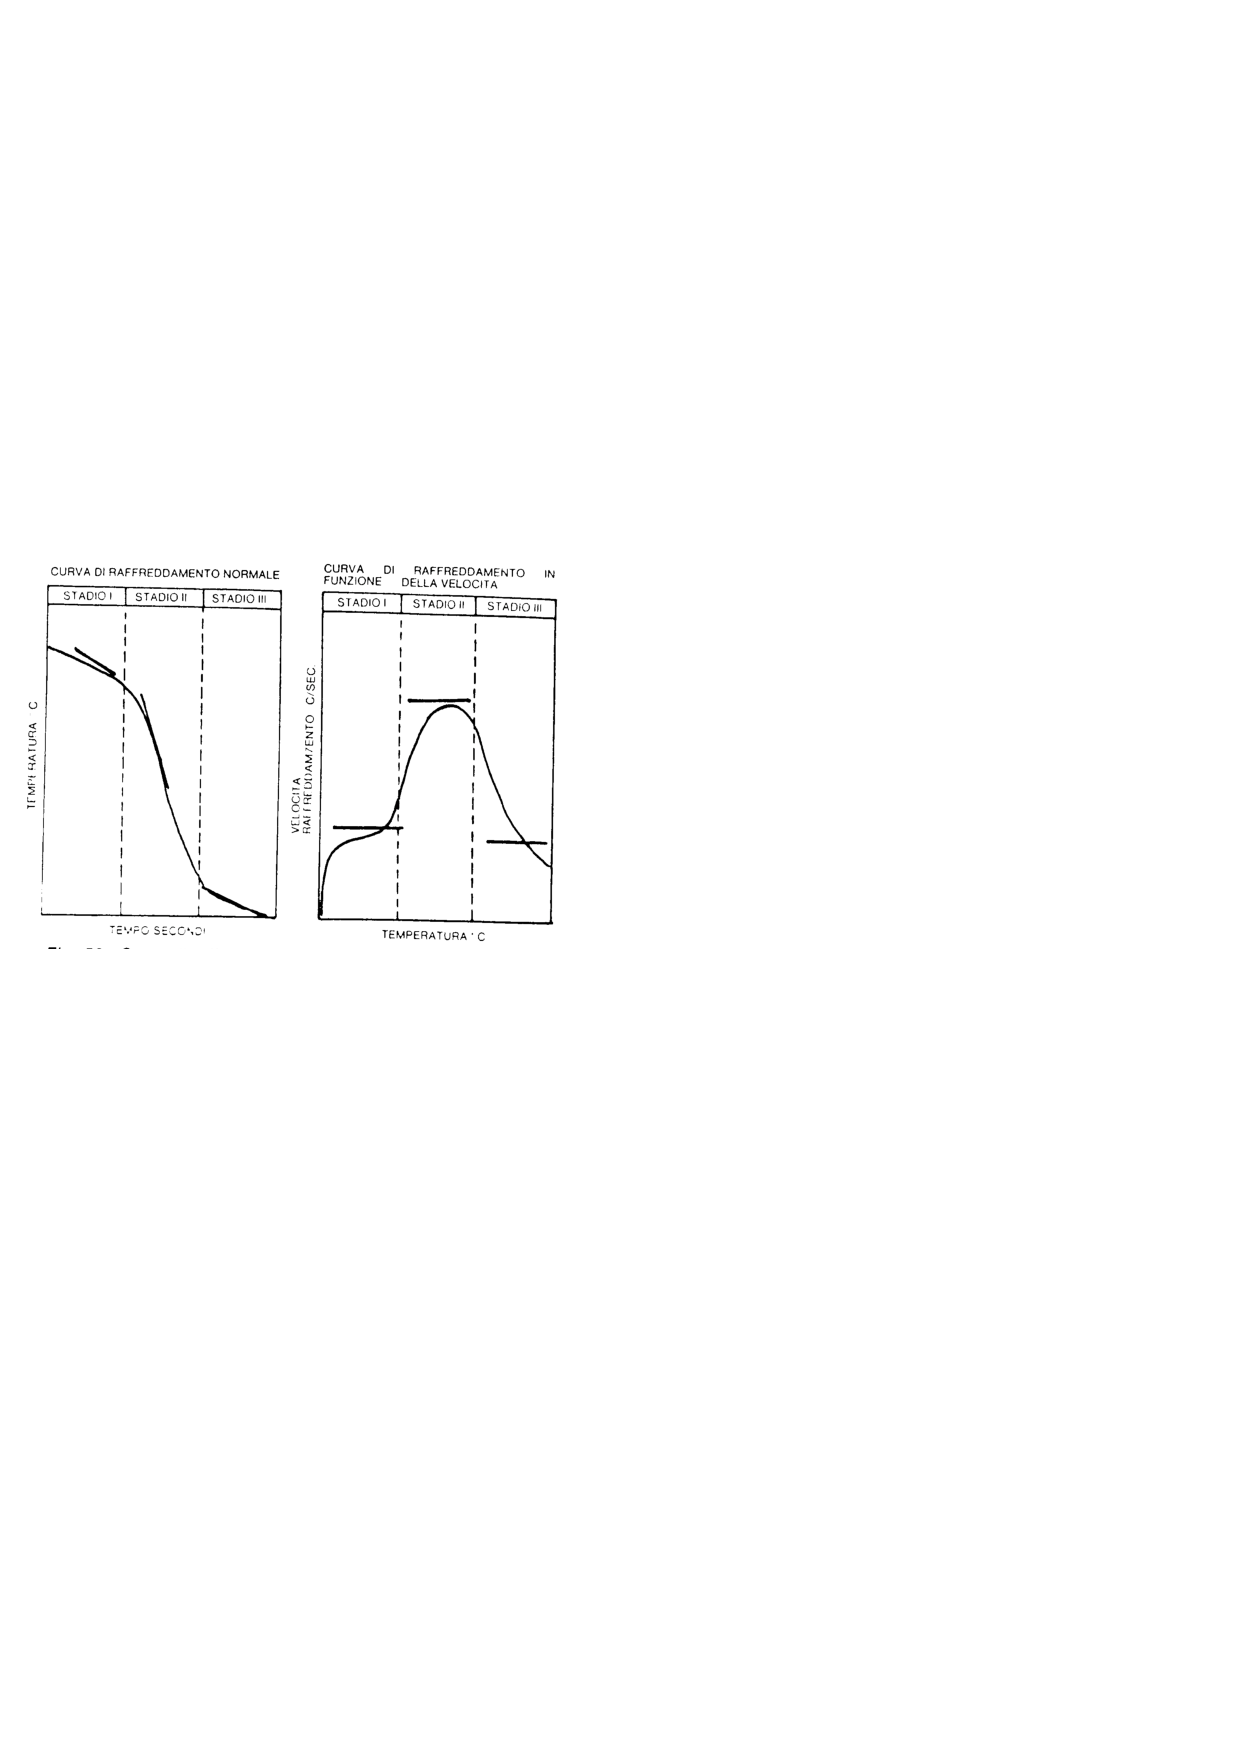
\includegraphics[width = 0.8\textwidth]{img42}
    \caption{Le tre fasi del raffreddamento per tempra}
    \labfig{img42}
\end{figure}

Per ottenere martensite in un acciaio eutettoidico bisogna trovarsi ad una temperatura di circa 550°C in meno di un secondo\sidenote{che sono le coordinate del gomito nel diagramma TTT}. Per raffreddare così velocemente si può utilizzare l’\textbf{acqua} che però presenta due problemi. Il primo è la \textbf{calefazione}: nel momento in cui si immerge il pezzo incandescente in acqua si forma una patina di vapore che isola lo isola. Il vapore conduce il calore molto meno dell'acqua liquida e si ottengono quindi dei tempi di raffreddamento più lunghi di quelli voluti.\\
Il secondo problema avviene quando si ha un’\textbf{elevata asportazione di calore} in presenza di un notevole gradiente, che favorisce la crescita di cricche. Tali gradienti elevati si hanno quando il cuore è caldo e la superficie è fredda. Per questo motivo si utilizzano gli \textbf{aqua quench}, che sono delle soluzioni alcoliche aggiunte all’acqua che hanno lo scopo di eliminare la guaina di vapore. Ciononostante quando si tempra in acqua c’è sempre il forte rischio di rompere il pezzo, per cui si cerca di non utilizzare l’acqua. Si usa per \textbf{acciai al solo carbonio} e \textbf{acciai da bonifica} (0,3 $\div$ 0,5 \%C).

L’altro fluido che viene utilizzato è l’\textbf{olio}, che ha un potere raffreddante inferiore a quello dell’acqua, ma non presenta calefazione. Gli \textbf{acciai} in questo caso devono essere \textbf{fortemente legati} poiché l’effetto degli elementi leganti (ad eccezione del cobalto) è quello di spostare a destra (cioè a tempi più lunghi) le curve TTT e CCT, e di conseguenza il gomito di formazione della martensite si ha anche per t=1000 s. Vi è così la possibilità di effettuare raffreddamenti più lenti. Tuttavia, l’olio inquina e sporca.\\
Gli elementi leganti sono di due tipi: quelli \textbf{austenitizzanti}, che stabilizzano la fase austenitica, cioè l’austenite sarà più lenta a trasformarsi, spostando le curve TTT a destra. Si tratta di Ni, Mn, N, Au; e quelli \textbf{ferritizzanti} (Cr, Ti, V, N) che, inoltre, hanno la caratteristica di formare carburi, con conseguente diffusione. Dato che però sono elementi estranei al reticolo, la loro diffusione è estremamente lenta e sposta le curve TTT verso destra.

L’austenite ottenuta tramite tempra (\textbf{quenched steel}) deve essere trattata ulteriormente tramite rinvenimento (\textbf{tempering}), ottenendo gli acciai da \textbf{bonifica}\index{bonifica} (temperated steel), cioè acciai sia temprati che rinvenuti.

Il \textbf{rinvenimento} si effettua in temperature di circa 500°C (450-500 °C), quindi al di sotto di \mathtext{A_3}, in tempi di circa un’ora e, per acciai speciali, si effettua anche due o tre volte.\\

\begin{figure}[!hbt]
    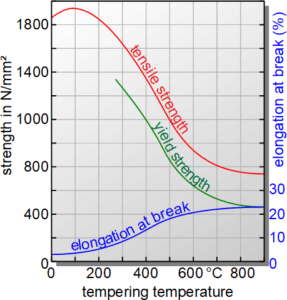
\includegraphics[width = 0.6\textwidth]{img39}
    \caption{Evoluzione delle caratteristiche meccaniche in funzione della temperatura di rinvenimento.}
    \labfig{img39}
\end{figure}

Oltre i 100°C l’austenite residua si trasforma in martensite. Contemporaneamente la martensite perde carbonio e da tetragonale diventa cubica. Si formano carburi di ferro metastabili $\varepsilon$ e $\chi$, e il reticolo diventa nuovamente CCC.\\
I carburi metastabili non sono carburi di equilibrio, ma sono due fasi coerenti, cioè hanno un’interfaccia comune con la matrice. Questo significa che i piani cristallografici sono simili a quelli della matrice e le dislocazioni, sebbene possano passare attraverso tali piani, incontrano della difficoltà, ottenendo così un rafforzamento notevole del materiale.

Dunque la presenza di carburi coerenti aumenta addirittura la durezza, come si può vedere nel diagramma HRC-T: la durezza aumenta fino a una temperatura di 200°C, quando i carburi si sciolgono nuovamente nella matrice, ottenendo ferrite e cementite e facendo diminuire la durezza.\\
Se l’acciaio è legato i carburi degli elementi legati, che sono coerenti possono dare vita a un fenomeno detto \textbf{indurimento secondario}, come si può vedere nella parte a destra del grafico. Tale indurimento è dovuto alla precipitazione dei carburi degli elementi leganti negli acciai legati (WC, TiC, MoC). Gli acciai legati hanno ottime proprietà meccaniche, come alta rigidezza (modulo di Young E) e alta tenacità.\\
Dopo il rinvenimento si ottiene una soluzione di ferrite e cementite con una struttura molto fine, tanto fine che al microscopio ottico non si riescono a distinguere le due fasi.

Gli \textbf{acciai bonificati} hanno elevate caratteristiche meccaniche e un’altissima tenacità.\\
Durante il rinvenimento però la tenacità crolla attorno ai 300°C, secondo il fenomeno della \textbf{fragilità da rinvenimento}, per un motivo ignoto. Vi sono però varie ipotesi: quella più plausibile è che visto che la matrice, ancora martensitica, è molto tensionata, la precipitazione dei carburi $\varepsilon$ e $\chi$ faccia crollare il valore della tenacità.\\

Per acciai da bonifica più pregiati, cioè temprati, si aggiunge il \textbf{molibdeno} in percentuali dallo 0,1 allo 0,2\%: in questo modo non si formano carburi $\varepsilon$ e $\chi$, ma carburi di molibdeno, che ha una maggiore affinità con il carbonio e che precipitano a temperature molto più elevate degli altri due. Dunque i carburi di molibdeno si formano quando la matrice è già detensionata.\\

Anche nelle \textbf{leghe di alluminio} viene effettuato il rinvenimento (indurimento), ma il meccanismo è differente.\\
Le leghe di alluminio sono classificate in base a un codice, a seconda degli elementi leganti:
\begin{itemize}
    \item 1000 alluminio puro;
    \item 2000 alluminio rame;
    \item 3000 alluminio manganese; \sidenote{Usati per serramenti}
    \item 4000 alluminio silicio;
    \item 5000 alluminio magnesio;
    \item 6000 alluminio magnesio silicio\sidenote{Telai delle automobili};
    \item 7000 alluminio zinco\sidenote{Usata in aeronautica, insieme alla serie 8000};
    \item 8000 alluminio litio.
\end{itemize}
Solo le serie 2000, 6000, 7000 e 8000 si prestano a trattamenti termici.

Nel caso di alluminio puro, l’unico metodo per aumentare le caratteristiche meccaniche è l’\textbf{incrudimento}.
Per le leghe sopra elencate, invece, è possibile intervenire con dei trattamenti termici con effetti simili a quelli che si ottengono sugli acciai.

\begin{figure}[!hbt]
    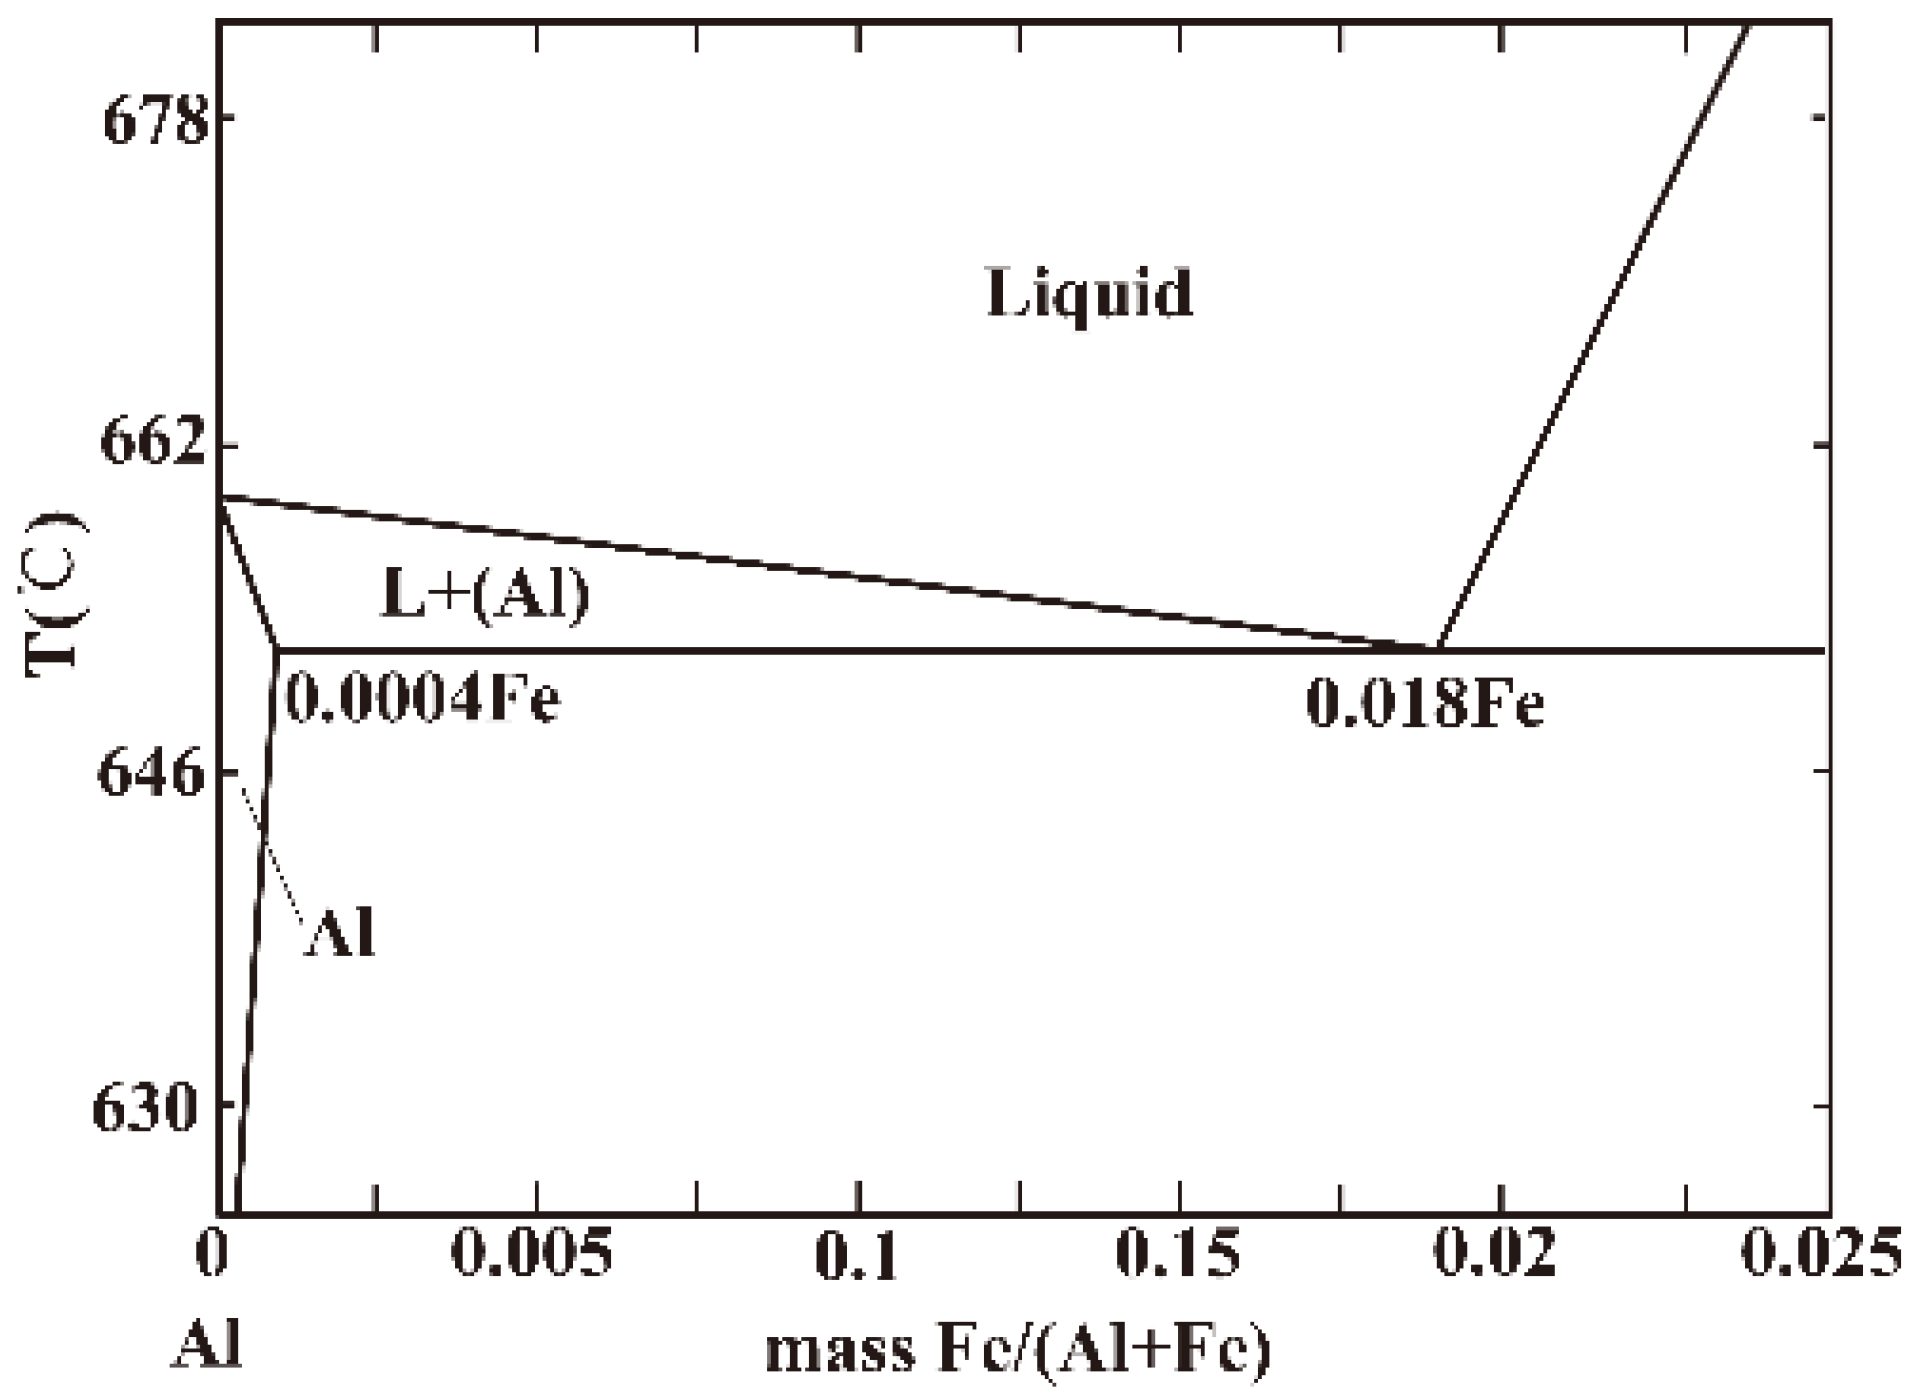
\includegraphics[width = 1\textwidth]{img38}
    \caption{Diagramma di stato AL-Fe. Questa medesima configurazione si può osservare in tutte le leghe di alluminio per bassi tenori di soluto.}
    \labfig{img38}
\end{figure}

Riscaldamento: si riscalda alla temperatura più alta possibile senza arrivare a liquefazione, quindi in prossimità della temperatura eutettica. Si ottiene quindi che tutto il soluto sia disciolto nella fase $\alpha$ (a sinistra nel diagramma).

Raffreddamento: se si raffredda lentamente, si segue il diagramma di stato e si forma la fase $\theta$, cioè il composto intermetallico (per esmpio \mathtext{Al_2Cu}), che è incoerente. Se si raffredda velocemente, ad esempio temprando in acqua, cioè non dando il tempo al soluto di diffondersi, si ottiene un fenomeno analogo a quello dell’austenite residua: si ottiene una soluzione solida di alta temperatura a temperatura ambiente, sovra-satura, che però non ha elevate caratteristiche meccaniche. 

Essendo fortemente metastabile, questa fase tende ad evolvere verso le condizioni di equilibrio, evoluzione che avviene a temperatura ambiente e in lassi di tempo molto lunghi, anche senza bisogno di ulteriori processi. Questo processo è detto \textbf{invecchiamento}: nell’arco di circa una settimana il rame (o chi per lui) che è presente si raggruppa in assembramenti (cluster), in cui è presente più rame di quello che è prevedibile su base statistica. Queste zone sono chiamate GP, termine che sta per \textbf{zone di Guinier-Preston}, distorcono la struttura, inducendo uno stato tensionale che sfavorisce il moto delle dislocazioni e aumenta quindi le caratteristiche meccaniche. Vi sono le zone GP1 e GP2. Sono seguite dalla formazione di altri composti metastabili, $\theta'$ e $\theta''$, seguiti dal composto di equilibrio $\theta$. Con la formazione di quest'ultimo si osserva un brusco crollo delle caratteristiche meccaniche, ed è dunque necessario arrestare il processo in una fase precedente.

L’invecchiamento quindi consiste nella far avvenire artificialmente (durata di qualche ora), cioè più velocemente, le trasformazioni GP1 e GP2 a temperature di 100-120°C, dopo un riscaldamento di 500°C.\\
Più aumenta la temperatura dell’invecchiamento artificiale più il tempo si riduce, andando a diminuire anche la durezza massima finale raggiungibile.\\
Quindi, Le fasi GP1, GP2 e $\theta'$ sono fasi coerenti che rafforzano notevolmente l’alluminio, ottenendo i DURAL, che presentano un carico di rottura molto elevato (dai 500 ai 650 MPa).\\
Il composto intermetallico coerente $\theta$’ assicura una continuità reticolare, poiché essendo coerente, non lascia buchi nel reticolo, come invece fanno le fasi incoerenti, come la fase $\theta$. Essa, tuttavia, non viene mai raggiunta perché essendo già a temperatura ambiente, i meccanismi diffusivi avverrebbero in un tempo infinito.\\
Se si formano il composto intermetallico $\theta$, cioè \mathtext{Al_2Cu}, vi è un crollo della durezza, dovuto proprio alla formazione di tale fase di equilibrio.\\
Discorso simile vale anche per le \textbf{leghe alluminio - titanio, alluminio-litio 8000, alluminio-zinco 7000, alluminio-magnesio-silicio 6000}.

Un altro trattamento termico per leghe di alluminio è la \textbf{solubilizzazione}\index{solubilizzazione}. Questo processo consiste nel riscaldamento di una lega ad una temperatura adeguata, mantenendo tale temperatura per un periodo sufficiente a causare la trasformazione di uno o più costituenti in una soluzione solida e quindi raffreddandola in modo sufficientemente rapido per mantenere tali costituenti nella soluzione.\\
La solubilizzazione viene in genere eseguita a temperature tra 450 e 575°C all’aria.

Le \textbf{leghe 4000 alluminio-silicio} sono leghe eupeptiche utilizzate per fare i pistoni. In questo caso, il rafforzamento non si ha per invecchiamento, ma durante la colata. Esse sono, infatti, considerate leghe da colata.\\
Il rafforzamento viene raggiunto aggiungendo delle piccole quantità di sodio, che spostano l’eutettico a temperature un po’ più basse, e con un tenore di silicio leggermente più elevato (da un tenore dell’11\% passiamo al 13\%), ottenendo il \textbf{punto eutettico modificato}.\\
Il vantaggio è quello di ottenere dei nuclei molto più piccoli, poiché si cola a temperature minori grazie all’aggiunta di sodio, realizzando una struttura finale più fine e con migliori caratteristiche meccaniche. Il silicio provoca la formazione dei nuclei di solidificazione a temperatura più bassa. Se i nuclei sono più fini di conseguenza si ottiene un alluminio con caratteristiche migliori. Inoltre, la presenza di silicio ipereutettico in grani conferisce un’elevata durezza al materiale, che infatti ha applicazioni nella costruzioni di pistoni e puntali da saldatura.\\

\section{Trattamenti superficiali}\index{trattamenti superficiali}
È possibile migliorare le caratteristiche meccaniche della superficie di un pezzo in acciaio senza modificarne il cuore tramite particolari trattamenti termici in atmosfere controllate. Questi processi vengono effettuati principalmente per aumentare la durezza e la resistenza alla fatica di componenti meccaniche, senza però dover rinunciare in toto alla tenacità che si accompagna a metalli più duttili.

\subsection{Cementazione}
A volte risulta desiderabile aumentare il tenore di carbonio della superficie di un pezzo, specialmente in acciai \textbf{a basso tenore di carbonio}. Questo processo, detto \textbf{cementazione}\index{cementazione} indurisce la superficie mantenendo il cuore del pezzo tenace. Inoltre l'inserimento di una maggior quantità di carbonio nel reticolo (in concentrazioni normalmente intorno allo 0,8\%) induce uno stato di compressione che consente di aumentare di molto la resistenza a fatica (in quanto aumenta la resistenza a trazione delle zone superficiali). \\
Il processo di cementazione avviene in atmosfere ricche di carbonio a temperature di circa 50°C superiori a quella di austenizzazione. Consta sostanzialemente di due fasi, ripetute fino all'ottenimento del tenore necessario di C:
\begin{enumerate}
    \item Boost: ovvero l'aumento vero e proprio del tenore di C. In questa fase si può superare lo 0,8\%;
    \item Diffusion: come avrà immaginato il lettore esperto della lingua dei sassoni, in questa fase si interrompe l'arricchimento per permettere al C di diffondersi verso gli strati più interni.
\end{enumerate}
Solitamente la zona interessata da questo tipo di trattamento è di qualche decimo di millimetro.\\
È possibile effettuare la cosiddetta cementazione diretta, in un'atmosfera di idrocarburi, attraverso la reazione:
\begin{equation*}
    \mathtext{C_xH_y \to C_{(\gamma)}+ H}
\end{equation*}
La formazione dell'idrogeno è, ovviamente, particolarmente pericolosa, sia per i potenziali effetti nocivi sulla resistenza del pezzo (si veda la sezione dedicata a pagina \pageref{problema idrogeno}) sia per l'alta infiammabilità della molecola.

\subsection{Nitrurazione}\index{nitrurazione}
Per ottenere un risultato analogo alla cementazione in acciai ferritici si usa il processo di nitrurazione, ovvero un trattamento termico superficiale in atmosfera di ammoniaca con lo scopo di introdurre N atomico nel reticolo dell'acciaio.\\
Il processo segue la reazione
\begin{equation*}
    \mathtext{2NH_3 \rightleftharpoons 2N_{(\alpha)} + 3H_2}
\end{equation*}
effettuata a circa 500°C per rimanere in campo ferritico, regolata dal potenziale di azoto (l'analogo del potenziale di carbonio definito a pagina \pageref{eq:PotC}) definito come:
\begin{equation*}
    \mathtext{p_N \propto \frac{p^2_{NH_3}}{p^3_{H_2}}}
\end{equation*}
In superficie si crea uno strato di qualche micrometro di nitruri duri e resistenti alla corrosione (\mathtext{Fe_4N} e \mathtext{Fe_2N}) detto \textbf{coltre bianca}, al disotto del quale si trova un strato (zona di diffusione) di ferrite $\alpha$ ricca in azoto.\\
La formazione delle varie fasi solide può essere studiata sul diagramma di Leher

\begin{figure}[!hbt]
    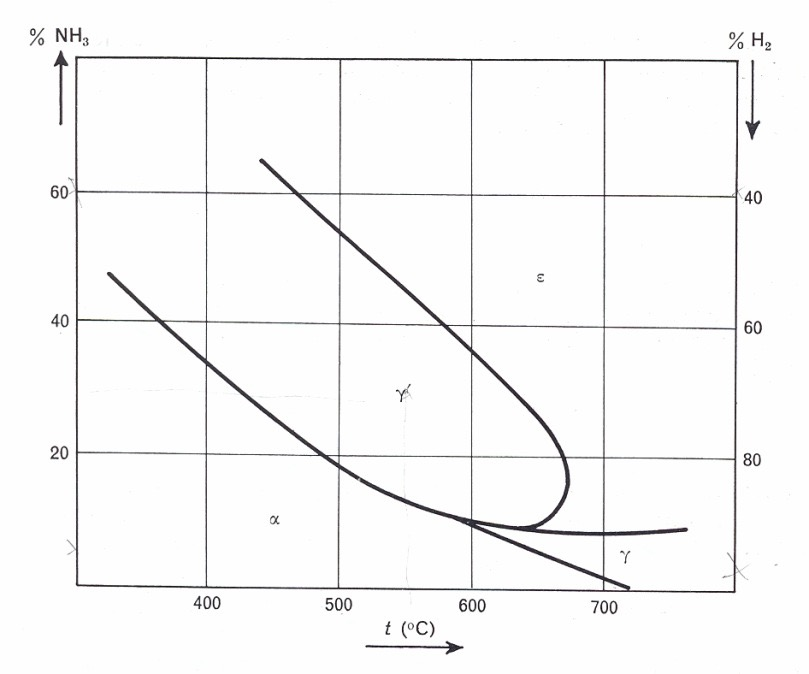
\includegraphics[width = 0.8\textwidth]{img37}
    \caption{Diagramma di Leher.}
\labfig{img37}
\end{figure}

Il processo richiede moltissimo tempo (circa 90 ore) e per questo è molto costoso. Viene quindi impiegato solo per pezzi finiti in acciai legati da bonifica.
Per aumentare la velocità è possibile usare un'atmosfera che combini ammoniaca e un gas cementante e aumentare la temperatura a 560°C\sidenote{È anche possibile usare dei bagni salini con cianuri o cianati}. Questo processo, detto \textbf{carbonitrurazione}\index{carbonitrurazione} richiede solo dall'una alle cinque ore, ma può portare alla formazione di composti sgraditi come N-austenite o N-martensite.

\subsection{Tempra superficiale}
È possibile temprare il pezzo soltanto in superficie adottando degli accorgimenti che impediscano al calore di penetrare in profondità. Questo processo può essere desiderabile perché la formazione di martensite, generando un aumento di volume degli strati esterni del pezzo, può dare indurre uno stato di compressione sulla superficie migliorando durezza e resistenza a fatica.\\
Il mezzo ad oggi più utilizzato consiste in un riscaldamento tramite induzione con un elettrodo percorso da corrente alternata, seguito da un immediato raffreddamento per mezzo di un getto d'acqua solidale all'elettrodo. Regolando frequenza e potenza della corrente è possibile regolare lo spessore della zona interessata dal trattamento ($f\uparrow$ spessore $\downarrow$, P $\uparrow$ spessore $\uparrow$).\\
Questo tipo di trattamento superficiale si usa per acciai da bonifica con tenori di carbonio compresi fra lo 0,3\% e lo 0,5\% già bonificati\sidenote{La presenza di grandi cristalli di ferrite e perlite crea problemi, perché le due strutture austenizzano a temperature diverse. La bonifica consente di lavorare con sfere finissime, che si comportano bene al riscaldamento}.